\documentclass[12pt]{article}

\setlength\parindent{0pt}

\usepackage[margin=0.8in]{geometry}
\usepackage{graphicx}
\usepackage{framed}
\usepackage[tiny]{titlesec}
\usepackage{amsmath}
%\usepackage[toc,page]{appendix}

%\titlespacing\section{0pt}{12pt plus 4pt minus 2pt}{0pt plus 2pt %minus 2pt}

\title{Fluid simulation}
\author{Valentin Miu}
\date{}

%\titleformat{\section}
%{\normalfont\medium\bfseries}{\thesection}{1em}{}

\makeatletter
\setlength{\@fptop}{0pt}
\makeatother

\begin{document}
\maketitle

\begin{abstract}
This essay presents summarizes several basic concepts of fluid simulations, discusses treatment of different types of fluids, and ...
\end{abstract}

\section{Introduction}

...history

\section{The Navier-Stokes equations}

Liquid fluids, and to a lesser extend gases, can be considered incompressible in most simulations. The behaviour of incompressible fluids are given by the Navier-Stokes equations (\ref{eq:NS1},~\ref{eq:NS2}):

\begin{equation}
\frac{\delta\vec{u}}{\delta t}+\vec{u}\cdot\nabla\vec{u}+\frac{1}{\rho}\nabla p=\vec{g}+\nu\nabla\cdot\nabla\vec{u}
\label{eq:NS1}
\end{equation}
\begin{equation}
\nabla\cdot\vec{u}=0
\label{eq:NS2}
\end{equation}

%[eulerian vs semi-lagrangian]

The Navier-Stokes equation can be solved from the Eulerian or Lagrangian viewpoints. In the former, the quantities are sampled at fixed points; in the latter, the quantities are sampled at the positions of particles moving with the flow (the ``snowman POV" and the ``snowflake POV", respectively). As a result, fluid simulations can be grid-based (for Eulerian) or particle-based (for Lagrangian). In many cases, the two are used in combination or in hybrid algorithms[2-way coupled SPH]. ()

\section{A simple grid-based Navier-Stokes simulation method}

The method used in [] is described. Due to the velocity divergence dependency, it is useful in grid-based simulations to use a staggered Marker-and-Cell (MAC) grid. This stores the pressure values at the centre of the grid cells, and the $xyz$-components of the velocity $\vec{u}$ (u, v, and w) at the centres of the grid walls (as in Figure \ref{fig:MACgrid}). This allows for the numerical computation of velocity divergence at the center of the cell, exactly where the pressure is sampled (\ref{eq:velDiv}. The velocity value itself at this point is determined by trilinear (linear in three dimensions) interpolation.

\begin{figure}[h]
\centering
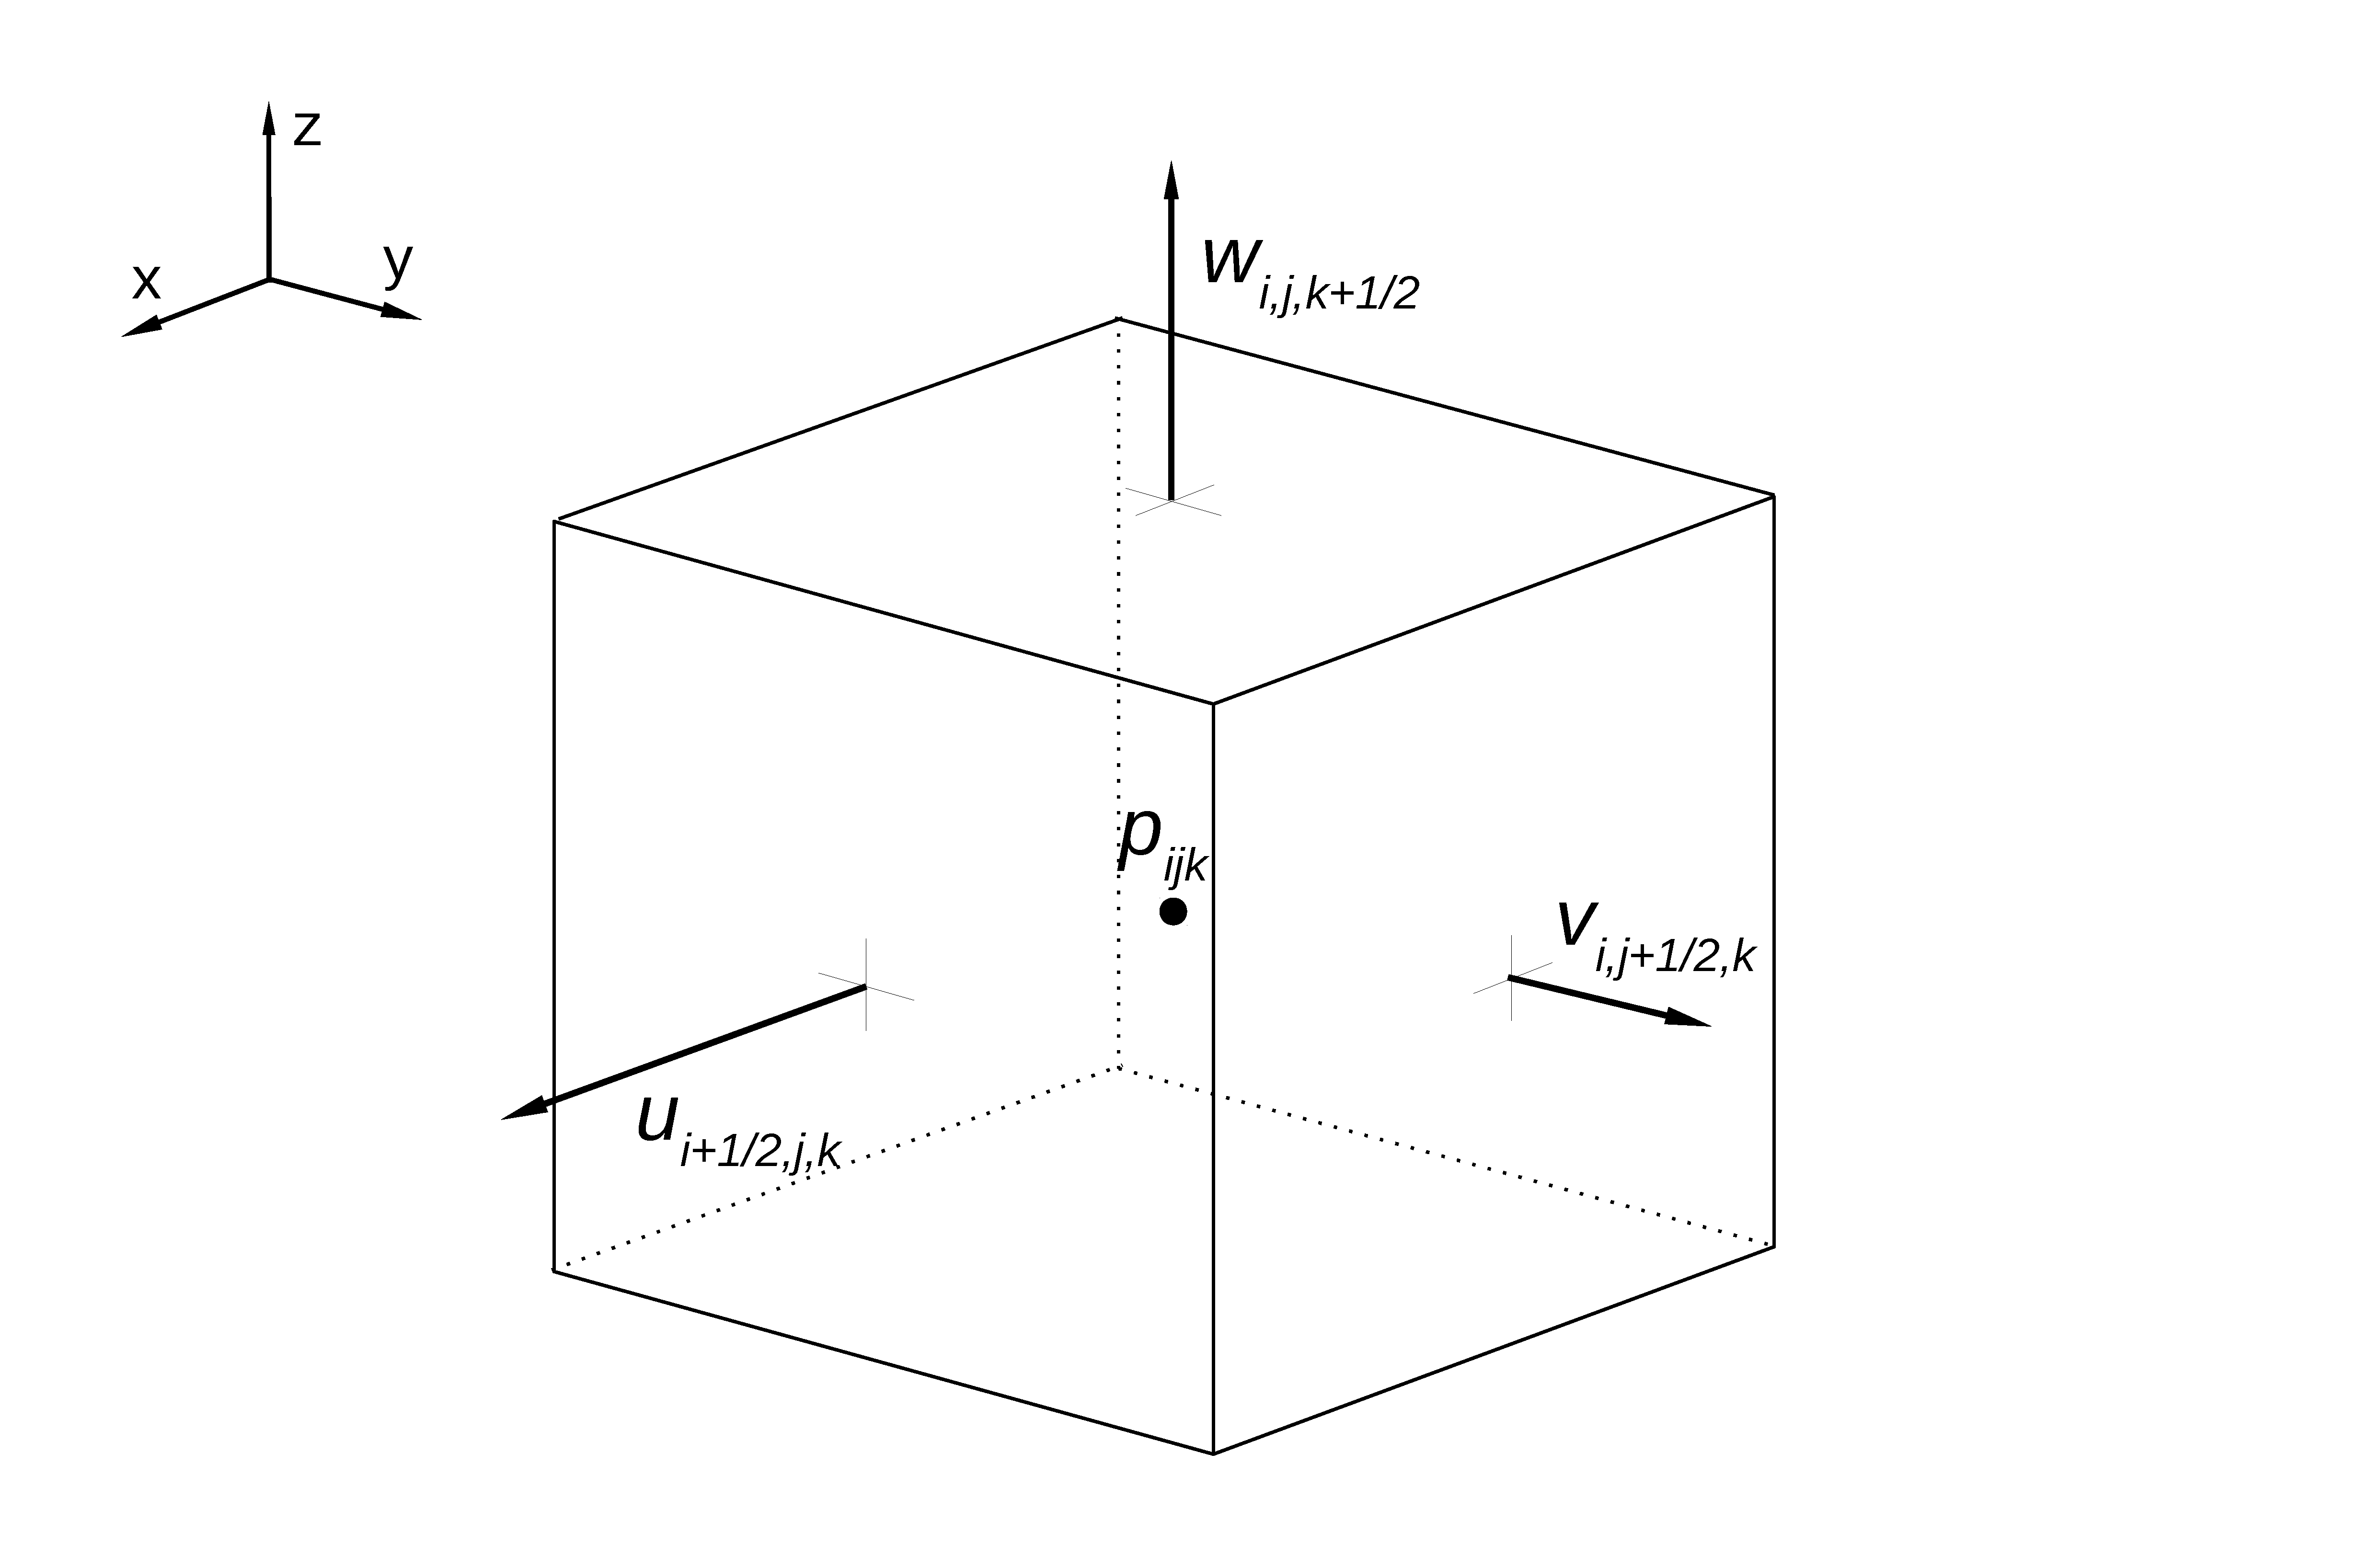
\includegraphics[width=0.7\linewidth]{mac_grid.pdf}
\caption{Data storage in one cell of a staggered MAC grid.}
\label{fig:MACgrid}
\end{figure}

\begin{equation}
\nabla\vec{u}_{i,j,k}\approx\frac{u_{i+\frac{1}{2},j,k}-u_{i-\frac{1}{2},j,k}}{2}+\frac{v_{i,j+\frac{1}{2},k}-v_{i,j-\frac{1}{2},k}}{2}+\frac{w_{i,j,k+\frac{1}{2}}-w_{i,j,k-\frac{1}{2}}}{2}
\label{eq:velDiv}
\end{equation}

Solving the Navier-Stokes equation can be simplified by breaking the equation down into three parts: the advection, body, and projection equations. Their respective processes \texttt{advect()}, \texttt{body()} and \texttt{project()} are applied in sequence for each time step.

When applied to the entire fluid, the advection equation enforces the conservation of energy (the fluid mass undergoes no net acceleration without the application of a net force). The \texttt{advect()} process applies the velocity field to the quantity $q$ for a time $dt$. This quantity may be velocity itself, pressure, or another quantity relevant to the particular fluid (such as temperature for smoke simulation).

Since in truth the fluid is acted on by the net force of gravity (and perhaps other forces), the body process simply adds $\vec{g}dt$ to the velocity field (all the members of the grid).

The incompressibility of the fluid is enforced by the \texttt{project()} process, which solves the Poisson equation by subtracting the correct pressure gradient from the output velocity grid of \texttt{body()} (\ref{eq:proj1}).

\begin{equation}
\vec{u}^{n+1}=\vec{u}_B^n-\Delta t\frac{1}{\rho}\nabla p
\label{eq:proj1}
\end{equation}

In numerical form, this results in a series of n equations, where n is the number of cells in the grid. If $\vec{p}$ is a column vector containing all the pressure unknowns, and $\vec{d}$ is a vector of the corresponding divergence values, the series of equations can be written as

\begin{equation}
Ap=d,
\label{eq:apd}
\end{equation}

where A is a symmetric sparse 3D matrix known as the seven-point Lagrangian matrix. This can be solved using the Modified Incomplete Cholesky Conjugate Gradient, Level Zero algorithm (MICCG(0)). This involves using the Preconditioned Conjugate Gradient algorithm (or PCG, shown in Figure \ref{fig:PCG}),

with the \texttt{applyPreconditioner()} function shown in Figure \ref{fig:precond}. Since $A$ is a symmetric sparse matrix with large-weight components only near and on the main diagonal, its storage can be optimized to $O(xSize*ySize*zSize)$ space.

If a fluid moves into a new space where the velocity has not been previously defined, it needs to be extrapolated from the nearest valid fluid cell. It is common for velocity to be sampled within a certain distance of the fluid surface in order to reduce such problems.

\section{Boundary conditions}

Fluid simulations are commonly expected to account for obstacles in the fluid volume. 

\section{Smoke}

Different types of fluids require specific considerations. For smoke, the body force is replaced with a temperature-dependent buoyancy force. Using the Boussinesq approximation of constant pressure, and assuming a linear dependence on only the temperature and smoke concentration.  (\ref{eq:fBuoy}

\begin{equation}
1+1=2
\label{eq:fBuoy}
\end{equation}

When using the semi-Lagrangian advection scheme, numerical dissipation leads to rapid destruction of the interesting features of smoke, such as vortices. This can be counteracted by creating a dependence on the vorticity $\vec{\omega}=\nabla\times\vec{u}$ (to boost vortex strength), or by using a sharper tricubic interpolant instead of the trilinear one.

\section{Water}

For the simulation of water, the issue of keeping track of the surface arises. The most basic method, suggested by Marker-and-Cell in 1965, involves using marker particles inside the grid volume. The presence of such a particle marks the presence of water at that point as the particles are moved by advection in the velocity field of the grid. However, this leads to poorly-defined, "blobby" water surfaces.

A superior method is the use of level sets. In their case, a function $\phi(x)$ is defined by values sampled at grid cells; the surface is described by $\phi(x) = 0$. This allows for easy modelling of smooth surfaces, as well as determining whether a point is inside the fluid volume, by simple interpolation to find the value of $\phi(x)$ at that point.

Since a given surface may be defined by multiple level sets, the function $\phi(x)$ offering the most stability is chosen. It is given by the gradient condition \ref{eq:phigrad}.

\begin{equation}
\|\nabla\phi(\vec{x})\|=1
\label{eq:phigrad}
\end{equation}

This is enforced by using the signed distance function for $\phi(x)$. (what is that?)

A caveat of level sets is that when combined with the advection process, numerical dissipation leads to the rapid destruction of small features (like small droplets or ripples). This can be solved by using par

\section{Smoothed Particle Hydrodynamics}

Although not nearly as computationally efficient in dealing with incompressible fluid volume, Smoothed Particle Hydrodynamics is far better than grid-based methods at creating visually pleasing fluid surfaces. While small interesting features like fine droplets and thin films are removed by numerical dissipation and limited resolution in grids, SPH is unaffected by these issues. As a result, modern fluid simulations use grid-based Navier-Stokes combined with SPH with particles seeded near fluid boundaries.

In SPH, every particle has an associated normalized smoothing kernel function $W(r)$, where r is the distance from the particle. To reduce computational cost, the function is given a cutoff point $r_c$ beyond which it is zero. Therefore, for one particle, only the particles in a vicinity of radius $r_c$ need to be considered.

A commonly used smoothing kernel is the poly6 kernel (\ref{eq:poly6}):

\begin{equation}
W_{poly6}(r)=\frac{315}{64\pi d^9}\cdot\begin{cases}
(r_c^2-r^2) & 0\leq r\leq r_c\\
0 & r>r_c\\
\end{cases}
\label{eq:poly6}
\end{equation}

SPH makes the Navier-Stokes equations trivial, as mass conservation can be enforced simply by keeping the number of particles constant. For liquid fluids, the boundary is again found through the level set method applied to the particle field.

%what is particle level set?

SPH is also useful in modelling compressible fluids such as sea foam, leading to impressive results if properly coupled with 

%Navier-Stokes and SPH can be used together by weighted influence based on the smoothed number density at a particle's position; the denser portion of the fluid is more affected by Navier-Stokes, while the more diffuse portions are more affected by SPH. This is known as particle slip.

%Grid-aided SPH methods can help in the simulation of dense and diffuse fluid mixtures and multiphase fluids. In the first case, a dependency on the number density of particles can be used to weigh the influence of Poisson solvers (the so).

\section{Other fluid simulation types}

For real-time simulations in games, the aforementioned methods are generally much too computationally expensive, although small-scale SPH methods are possible (the chinese dude citation).

Heightfield approximations use the two-dimensional wave equation as a displacement map in the z direction. This however does not allow for multiple z solutions per (x,y) point, as a breaking wave would for example require.

Ocean surfaces can also be generated using procedural animation, as the sum of various sinusoidal functions of varying direction, amplitude, and frequency. This is not well suited for interaction with boundaries or solid objects in the water; this shortcoming can be obfuscated by texturing foam onto the mesh near obstacles and/or using particle emitters.

These types of simulation are far less computationally expensive than 3D Navier-Stokes methods; this makes them suitable for real-time simulations in games. Still, small-scale SPH can also be used in real-time [chinese guy citation], and so can grid-based methods (by using the Jacobi method in the projection step.

\section{Fluid simulations through deep learning}

The most computationally demanding step of fluid simulations is projection. This has recently been shown to be surprisingly well handled by neural networks trained on exact fluid solvers, even when the initial conditions of fluid in the solver and network differ. Furthermore, unlike traditional exact solvers, the complexity of this approach is not dependent on boundary conditions.

[maybe put a picture here reflecting it]

\section*{Annex}
\renewcommand{\thefigure}{A\arabic{figure}}

\setcounter{figure}{0}

\begin{figure}[h]
\begin{framed}
\texttt{// "$\cdot$" is the dot product of two vectors; "*" is scalar multiplication}

\texttt{p = 0}

\texttt{r = d}

\texttt{z = applyPreconditioner(r)}

\texttt{s = z}

\texttt{$\sigma$ = z $\cdot$ r}

\texttt{iterations = 0}

\texttt{while (p not within tolerance) and (iterations < maximumIterations)}

\texttt{~~~~z = A $\cdot$ s}

\texttt{~~~~$\alpha$ = $\rho$ / (z $\cdot$ s)}

\texttt{~~~~p = p + $\alpha$ * s}

\texttt{~~~~r = r - $\alpha$ * z}

\texttt{~~~~// if the element of r with the greatest absolute value is within}

\texttt{~~~~// tolerance, take current p as the solution}

\texttt{~~~~if (max(|r|) $\leq$ tol) return p}

\texttt{~~~~$\sigma_{new}$ = z $\cdot$ r}

\texttt{~~~~$\beta$ = $\sigma_{new}$ / $\rho$}

\texttt{~~~~s = z + $\beta$ * s}

\texttt{~~~~$\sigma$ = $\sigma_{new}$}

\texttt{// maximum iterations have been exceeded}

\texttt{return r} 

\end{framed}
%\centering
\vspace*{-3mm}\caption{The PCG algorithm.}
\label{fig:PCG}
\end{figure}

\begin{figure}[h]
\begin{framed}
\texttt{//set tuning constant}

\texttt{$\tau$ = 0.97}

\texttt{}

\texttt{//calculate the preconditioner}

\texttt{for i = 1 to xSize, j = 1 to ySize, k = 1 to zSize}

\texttt{~~if (grid cell has fluid in it)}

\texttt{~~~~e = A$_{(i,j,k)(i,j,k)}$ - (A$_{(i+1,j,k)(i-1,j,k)}$ * precon$_{i-1,j,k}$)$^2$}

\texttt{~~~~~~~~~~~~~~~~~- (A$_{(i,j+1,k)(i,j-1,k)}$ * precon$_{i,j-1,k}$)$^2$} 

\texttt{~~~~~~~~~~~~~~~~~- (A$_{(i,j,k+1)(i,j,k-1)}$ * precon$_{i,j,k-1}$)$^2$}

\texttt{~~~~~~~~~~~~~- $\tau$ * (A$_{(i+1,j,k)(i-1,j,k)}$ * (A$_{(i,j+1,k)(i-1,j,k)}$ + A$_{(i,j,k+1)(i-1,j,k)}$) * precon$_{i-1,j,k}^2$}

\texttt{~~~~~~~~~~~~~- $\tau$ * (A$_{(i,j+1,k)(i,j-1,k)}$ * (A$_{(i+1,j,k)(i,j-1,k)}$ + A$_{(i,j,k+1)(i,j-1,k)}$) * precon$_{i,j-1,k}^2$}

\texttt{~~~~~~~~~~~~~- $\tau$ * (A$_{(i,j,k+1)(i,j,k-1)}$ * (A$_{(i+1,j,k)(i,j,k-1)}$ + A$_{(i,j+1,k)(i,j,k-1)}$) * precon$_{i,j,k-1}^2$}

\texttt{}

\texttt{//Solve Lq = r}

\texttt{for i = 1 to xSize, j = 1 to ySize, k = 1 to zSize}

\texttt{~~if (grid cell has fluid in it)}

\texttt{~~~~t = r$_{i,j,k}$ - A$_{(i+1,j,k)(i-1,j,k)}$ * precon$_{i-1,j,k}$ * q$_{i-1,j,k}$}

\texttt{~~~~~~~~~~~~~- A$_{(i,j+1,k)(i,j-1,k)}$ * precon$_{i,j-1,k}$ * q$_{i,j-1,k}$}

\texttt{~~~~~~~~~~~~~- A$_{(i,j,k+1)(i,j,k+1)}$ * precon$_{i,j,k-1}$ * q$_{i,j,k-1}$}

\texttt{~~~~q$_{i,j,k}$ = t * precon$_{i,j,k}$}

\texttt{}

\texttt{//Solve L$^T$z = q}

\texttt{for i = xSize to 1, j = ySize to 1, k = zSize to 1}

\texttt{~~if (grid cell has fluid in it)}

\texttt{~~~~t = r$_{i,j,k}$ - A$_{(i,j,k)(i,j,k)}$ * precon$_{i,j,k}$ * z$_{i+1,j,k}$}

\texttt{~~~~~~~~~~~~~- A$_{(i,j,k)(i,j,k)}$ * precon$_{i,j,k}$ * q$_{i,j+1,k}$}

\texttt{~~~~~~~~~~~~~- A$_{(i,j,k)(i,j,k)}$ * precon$_{i,j,k}$ * q$_{i,j,k+1}$}

\texttt{~~~~z$_{i,j,k}$ = t * precon$_{i,j,k}$}

\end{framed}
\centering
\vspace*{-3mm}\caption{An optimized preconditioner corresponding to the weighted average ($\tau$=97\%) between MICCG(0) and regular Incomplete Cholesky (ICCG(0)).}
\label{fig:precond}
\end{figure}

%\begin{thebibliography}
%\end{thebibliography}


\end{document}